\section{Supplementary \texorpdfstring{$L(2,1)$}{L(2,1)} symmetry experiments}\label{sec:legacy-experiments}
\subsection{Data sources and completeness checks}
These symmetry experiments use two completed runs:
\begin{itemize}
\item \path{results/runs/cycles_main_r1.csv}: $C_n$ with
$\CycleFirst\leq n\leq\CycleLast$, comprising \CycleCount{} graphs;
\item \path{results/runs/products_main_r1.csv}: seven product families with
$\ProductFirst\leq n\leq\ProductLast$ and
$\ProductMFirst\leq m\leq\ProductMLast$, comprising \ProductCount{} graphs.
\end{itemize}
Each row pairs Baseline and Symmetry on the same graph. There are
\ComparisonCount{} pairs, corresponding to \WitnessCount{} runs. Historical
CSVs are retained for reference but are not pooled into the following tables
or figures. The historical Petersen sweep and older ILP results are not
baselines for these two runs.

Each CSV has a configuration/source/environment manifest and a JSONL file
containing incumbent labels, lower bounds, span-search history, and counters
for completed trials. The exporter checks graph names against the sweep
domain, absence of missing or duplicate rows, equal spans in every OPT/OPT
pair, and consistency between witnesses and CSV rows. All \WitnessCount{}
labelings are rechecked by traversing edges and two-step paths. Under the
matching historical source version, both CNFs are rebuilt at
\texttt{Count\_Span} to verify variable, raw-clause, and simplified-clause
counts without solving SAT. CSV, manifest, witness, and exporter hashes
are stored in \path{paper/generated/sources.json}. Labeling checks do not
independently verify UNSAT conclusions; DRAT/LRAT certificates are not exported.

\subsection{Configuration and measurement definitions}
\begin{table}[H]
\caption{Archived symmetry-run configurations.}
\centering\small% Generated from main runs; do not edit numbers manually.
\begin{tabular}{llrllr}
\toprule
Dataset & $n$ range & Pairs & Solver & Search & Budget (s) \\
\midrule
Chu trình & 3--50 & 48 & glucose & hybrid & 60 \\
Product & 3--10 & 448 & glucose & hybrid & 180 \\
\bottomrule
\end{tabular}

\tablenote{Configuration from the manifests. For products, the $m$ range is
$\ProductMFirst$--$\ProductMLast$; the budget applies to each configuration
on each graph.}
\end{table}
Both runs used Python 3.13.7, NetworkX 3.6.1, and PySAT 1.9.dev15 on the
recorded macOS 13.7.8 x86\_64 environment. CPU, RAM, and background-load
information was not fully recorded, so timings are not machine-independent
characteristics. The option name \texttt{hybrid} is retained for CLI
compatibility; span selection uses the interval midpoint, i.e., binary search,
with a fresh solver per trial. Base/Sym order alternates by instance;
both runs use \texttt{order\_offset=0}.

Baseline and Symmetry share the encoder and common preprocessing. Only $C_n$
fixes $f(0)=0$, combined with reflection-based neighbor ordering; these
experiments do not isolate the effects of the two constraints. Products do
not use root fixing. Families marked ``None added'' use the same model in
both runs and measure repeated-run variation, not a new symmetry-breaking technique.

\texttt{Time\_*} includes preprocessing, process startup, CNF construction,
search, validation, and cleanup. The deadline applies to the search process;
preprocessing and cleanup may cause slight overruns. Rebuilding the two
CNFs for size measurement is outside these runtimes.
\texttt{Encoding\_Time} and \texttt{SAT\_Solve\_Time} sum completed trials
only and do not include all overhead.

\texttt{Count\_Span} is the larger incumbent span. When both runs establish
the same optimum, it is the optimal span; otherwise, it is only a common
feasible upper bound. \texttt{Clause\_Raw\_*} is counted after root-constant
substitution and before common preprocessing; \texttt{Clause\_*} is counted
after preprocessing, including retained units. Variable counts refer to
allocated variables, not those left unassigned by propagation. These are
input CNF counts, not counts after backend preprocessing or clause learning.

\subsection{Optimality coverage and unresolved instances}
\begin{table}[H]
\caption{Symmetry-run coverage by family.}
\centering\small\setlength{\tabcolsep}{4pt}
% Generated from main runs; do not edit numbers manually.
\begin{tabular}{lrrrrl}
\toprule
Family & Pairs & OPT/OPT & Unresolved & Span (OPT) & Symmetry \\
\midrule
$C_n$ & 48 & 48 & 0 & 4 & Root + order \\
$C_n \mathbin{\square} C_m$ & 64 & 62 & 2 & 6--8 & Order \\
$C_n \mathbin{\square} P_m$ & 64 & 64 & 0 & 6--7 & Order \\
$P_n \mathbin{\square} P_m$ & 64 & 64 & 0 & 6 & None added \\
$C_n \circ C_m$ & 64 & 64 & 0 & 7--14 & Order \\
$C_n \circ P_m$ & 64 & 64 & 0 & 7--14 & Order \\
$P_n \circ C_m$ & 64 & 64 & 0 & 7--14 & None added \\
$P_n \circ P_m$ & 64 & 64 & 0 & 6--14 & None added \\
\bottomrule
\end{tabular}

\tablenote{Results by family. Span ranges include only matching OPT/OPT
pairs; ``Unresolved'' counts pairs with at least one run lacking an optimality conclusion.}
\end{table}
There are \PairedOpt{} jointly OPT pairs, with no span disagreements.
Every cycle in the evaluated domain has span 4. Two product instances
remain unresolved under both configurations:
$C_9\mathbin{\square}C_{10}$ and $C_{10}\mathbin{\square}C_9$.
\begin{table}[H]
\caption{Unresolved symmetry-run intervals.}
\centering\small% Generated from main runs; do not edit numbers manually.
\begin{tabular}{lrrrrr}
\toprule
Graph & $L_B$ & $U_B$ & $L_S$ & $U_S$ & Count span \\
\midrule
$C_{9}\mathbin{\square}C_{10}$ & 5 & 10 & 5 & 10 & 10 \\
$C_{10}\mathbin{\square}C_{9}$ & 7 & 8 & 7 & 8 & 8 \\
\bottomrule
\end{tabular}

\tablenote{Bound intervals $[L,U]$ for FEASIBLE runs; each $U$ has an explicit
labeling. Bounds come from witnesses, not from an unproved formula.}
\end{table}
These graphs are isomorphic by coordinate exchange. Incumbents can differ
because of vertex order and search history; their upper bounds are not two
optimal values. For $C_9\mathbin{\square}C_{10}$, both runs were interrupted
before completing a span trial, so recorded zero counters do not mean the
solver performed no work. All four FEASIBLE runs have
\texttt{Stats\_Complete=False}.

\subsection{CNF size and runtime by family}
Let $t_B,t_S$ denote the two runtimes. A ratio $t_B/t_S>1$ indicates a faster
Symmetry run for that pair. The following tables use jointly OPT pairs only.
FEASIBLE pairs are reported separately and are not assigned substitute runtimes.
\begin{table}[H]
\caption{Runtime comparison on jointly OPT pairs.}
\centering\small% Generated from main runs; do not edit numbers manually.
\begin{tabular}{lrrrr}
\toprule
Family & OPT/OPT & $\sum t_B$ (s) & $\sum t_S$ (s) & Median $t_B/t_S$ \\
\midrule
$C_n$ & 48 & 22.987 & 23.983 & 1.000 \\
$C_n \mathbin{\square} C_m$ & 62 & 326.842 & 131.803 & 1.103 \\
$C_n \mathbin{\square} P_m$ & 64 & 39.972 & 38.580 & 1.021 \\
$P_n \mathbin{\square} P_m$ & 64 & 35.113 & 35.582 & 1.000 \\
$C_n \circ C_m$ & 64 & 769.385 & 447.613 & 1.120 \\
$C_n \circ P_m$ & 64 & 701.840 & 497.427 & 1.112 \\
$P_n \circ C_m$ & 64 & 402.675 & 402.658 & 0.992 \\
$P_n \circ P_m$ & 64 & 402.654 & 405.998 & 1.005 \\
\bottomrule
\end{tabular}

\tablenote{Total runtimes and median ratios on jointly OPT pairs. Total time
and the median of pairwise ratios are different statistics.}
\end{table}
\begin{table}[H]
\caption{Variable and clause reductions.}
\centering\small\setlength{\tabcolsep}{4pt}% Generated from main runs; do not edit numbers manually.
\begin{tabular}{lrrrrr}
\toprule
Family & Var. reduction (\%) & Clause reduction (\%) & Fewer & Equal & More \\
\midrule
$C_n$ & 3.77 & 12.58 & 48 & 0 & 0 \\
$C_n \mathbin{\square} C_m$ & 0.00 & 0.83 & 62 & 0 & 0 \\
$C_n \mathbin{\square} P_m$ & 0.00 & 0.58 & 64 & 0 & 0 \\
$P_n \mathbin{\square} P_m$ & 0.00 & 0.00 & 0 & 64 & 0 \\
$C_n \circ C_m$ & 0.00 & 1.11 & 64 & 0 & 0 \\
$C_n \circ P_m$ & 0.00 & 1.14 & 64 & 0 & 0 \\
$P_n \circ C_m$ & 0.00 & 0.00 & 0 & 64 & 0 \\
$P_n \circ P_m$ & 0.00 & 0.00 & 0 & 64 & 0 \\
\bottomrule
\end{tabular}

\tablenote{Median percentage reductions in variables and clauses. The final
three columns count pairs with fewer/equal/more Symmetry clauses than Baseline.
The subset is the same OPT/OPT subset as in the runtime table.}
\end{table}
For cycles, the median clause reduction is \CycleClauseMedian\%, whereas
the median $t_B/t_S$ is only \CycleTimeRatio. These small instances incur
substantial startup and non-SAT overhead. This single-run dataset does not
show a clear total-runtime benefit from the reduced CNF size.

For jointly OPT $C_n\mathbin{\square}C_m$ pairs, the median ratio is
\CxCTimeRatio, while the ratio of total runtimes is \CxCTotalTimeRatio.
The difference indicates that totals are more sensitive to a few expensive
instances. For $C_n\circ C_m$ and $C_n\circ P_m$, median ratios are
\CoCTimeRatio{} and \CoPTimeRatio, respectively. These are observed gains
in this run, not established improvements across repeated runs.
$P_n\mathbin{\square}P_m$, $P_n\circ P_m$, and $P_n\circ C_m$ add no
family-specific symmetry constraints; timing differences reflect measurement variation.

\begin{figure}[htbp]
\centering
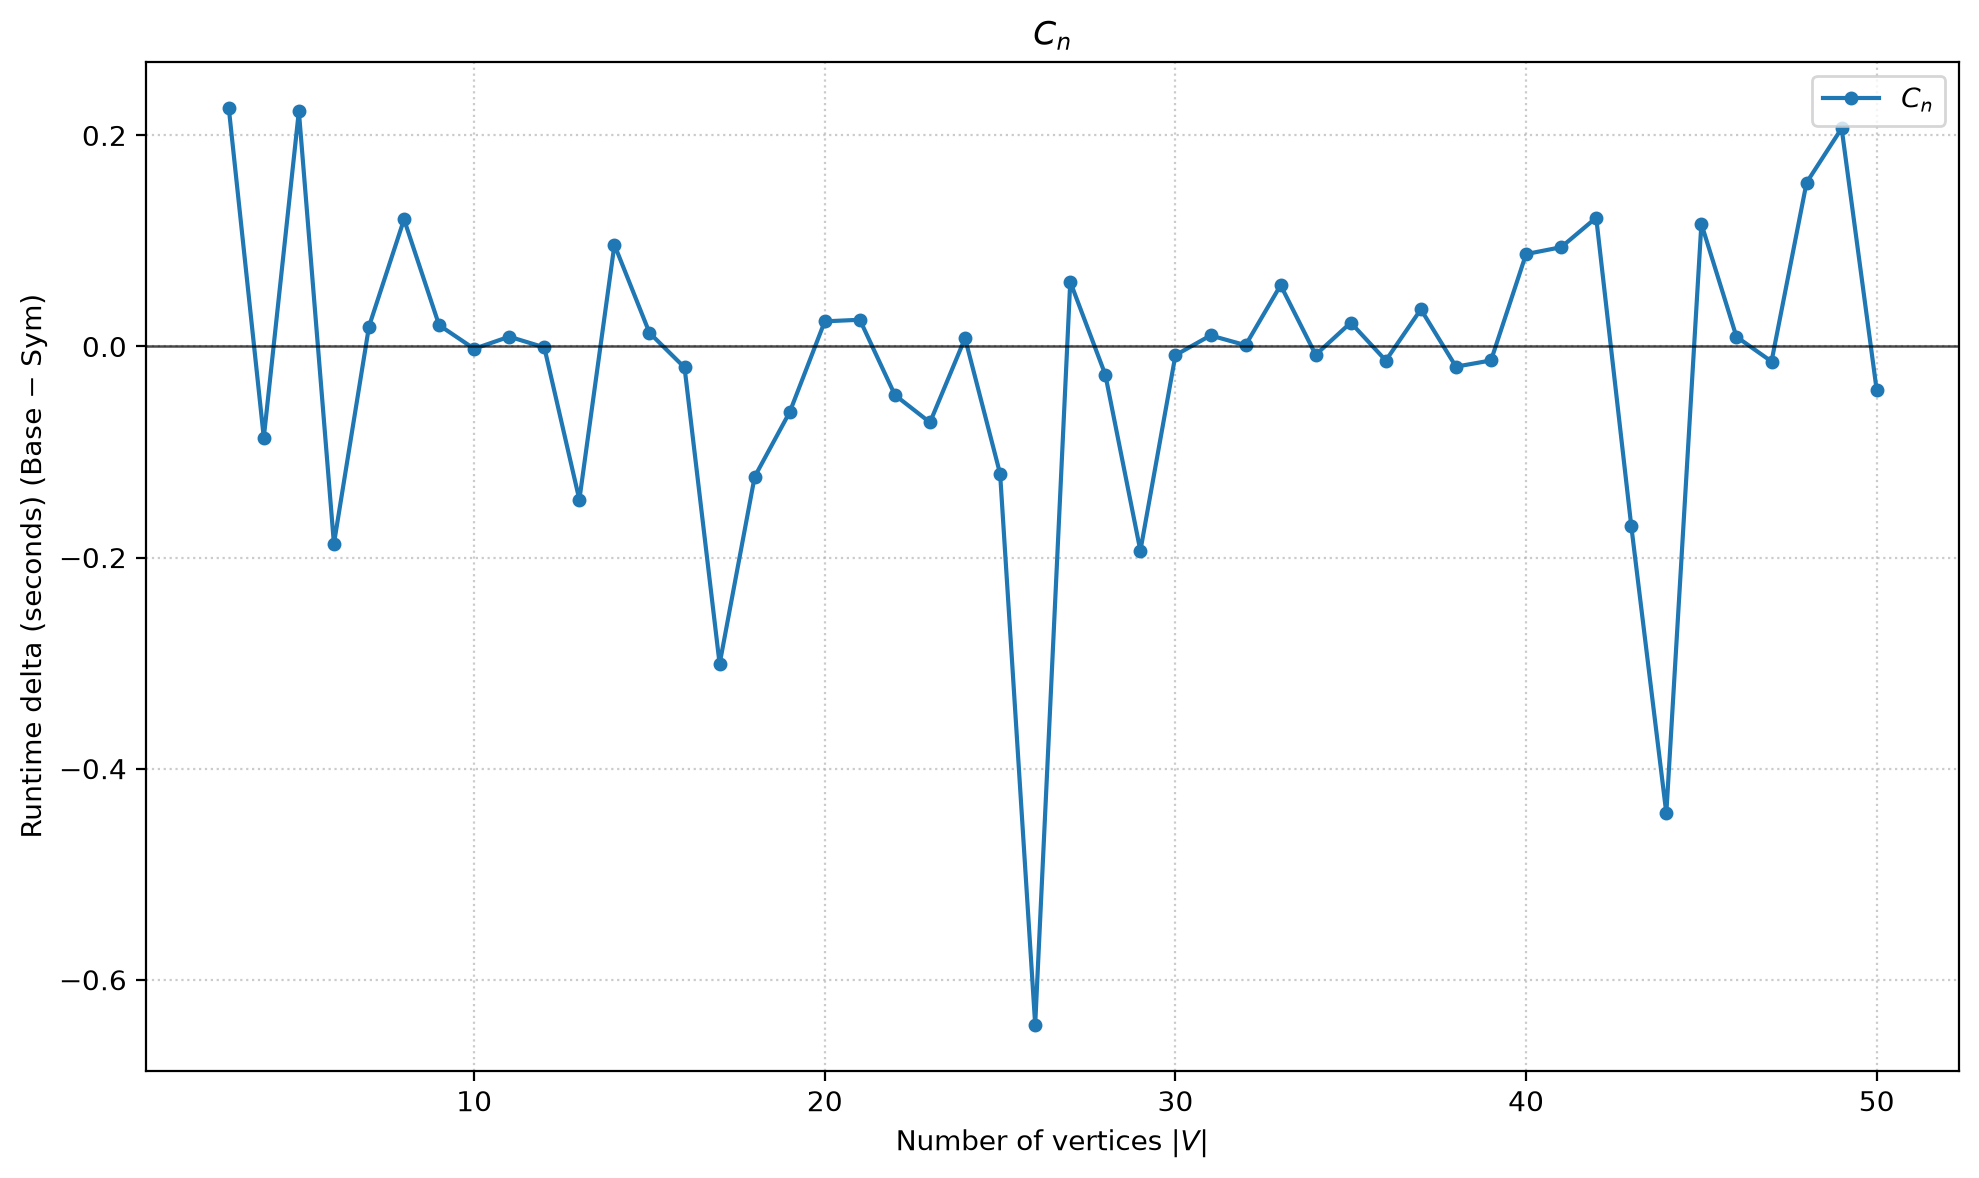
\includegraphics[width=0.49\linewidth]{paper/generated/cycles_main_r1_plots/delta_runtime_C.png}
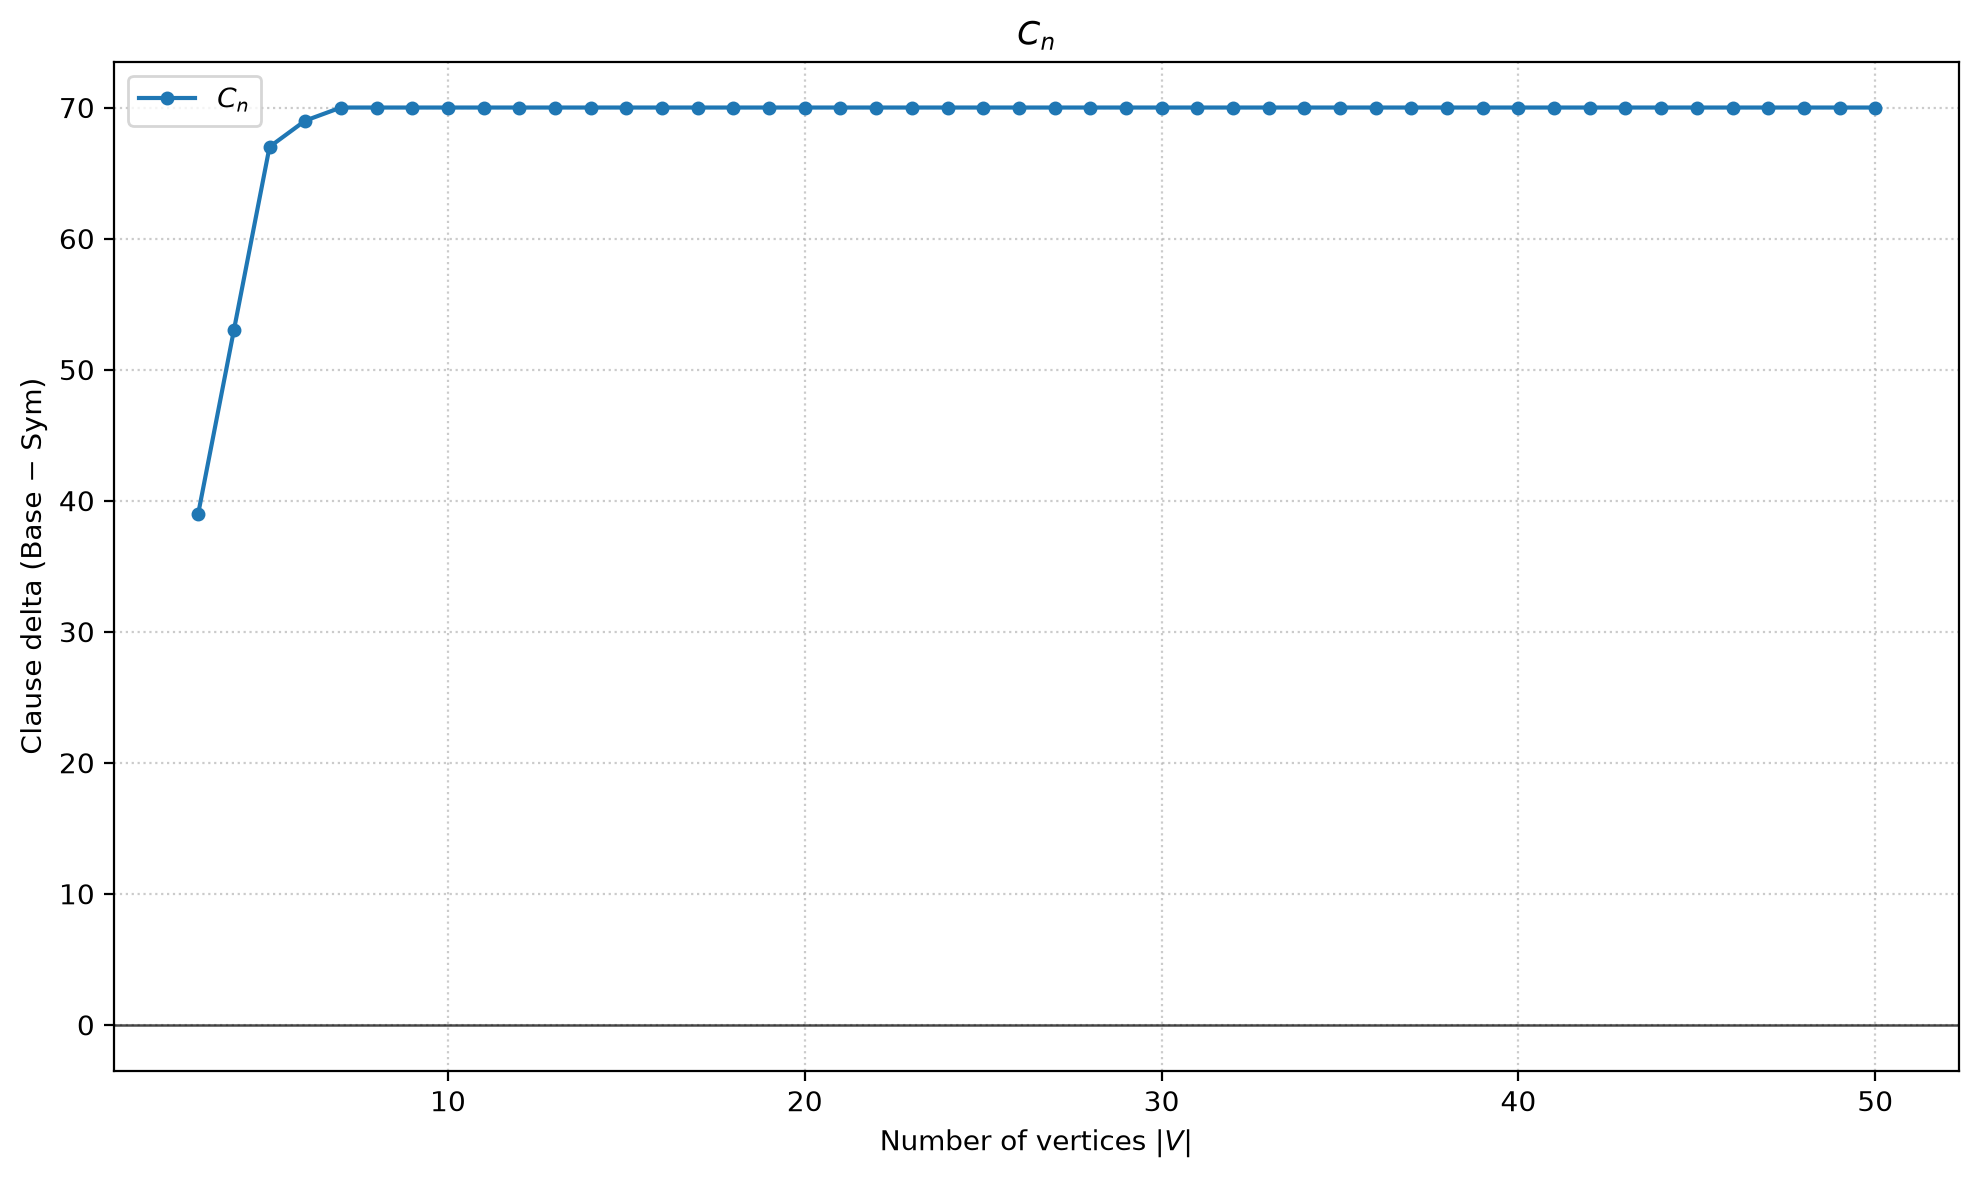
\includegraphics[width=0.49\linewidth]{paper/generated/cycles_main_r1_plots/delta_clauses_C.png}
\caption{Symmetry effects on cycles.}
\tablenote{Cycles: runtime and clause differences, Base minus Sym. Negative
runtime differences indicate slower Symmetry runs.}
\end{figure}
\begin{figure}[htbp]
\centering
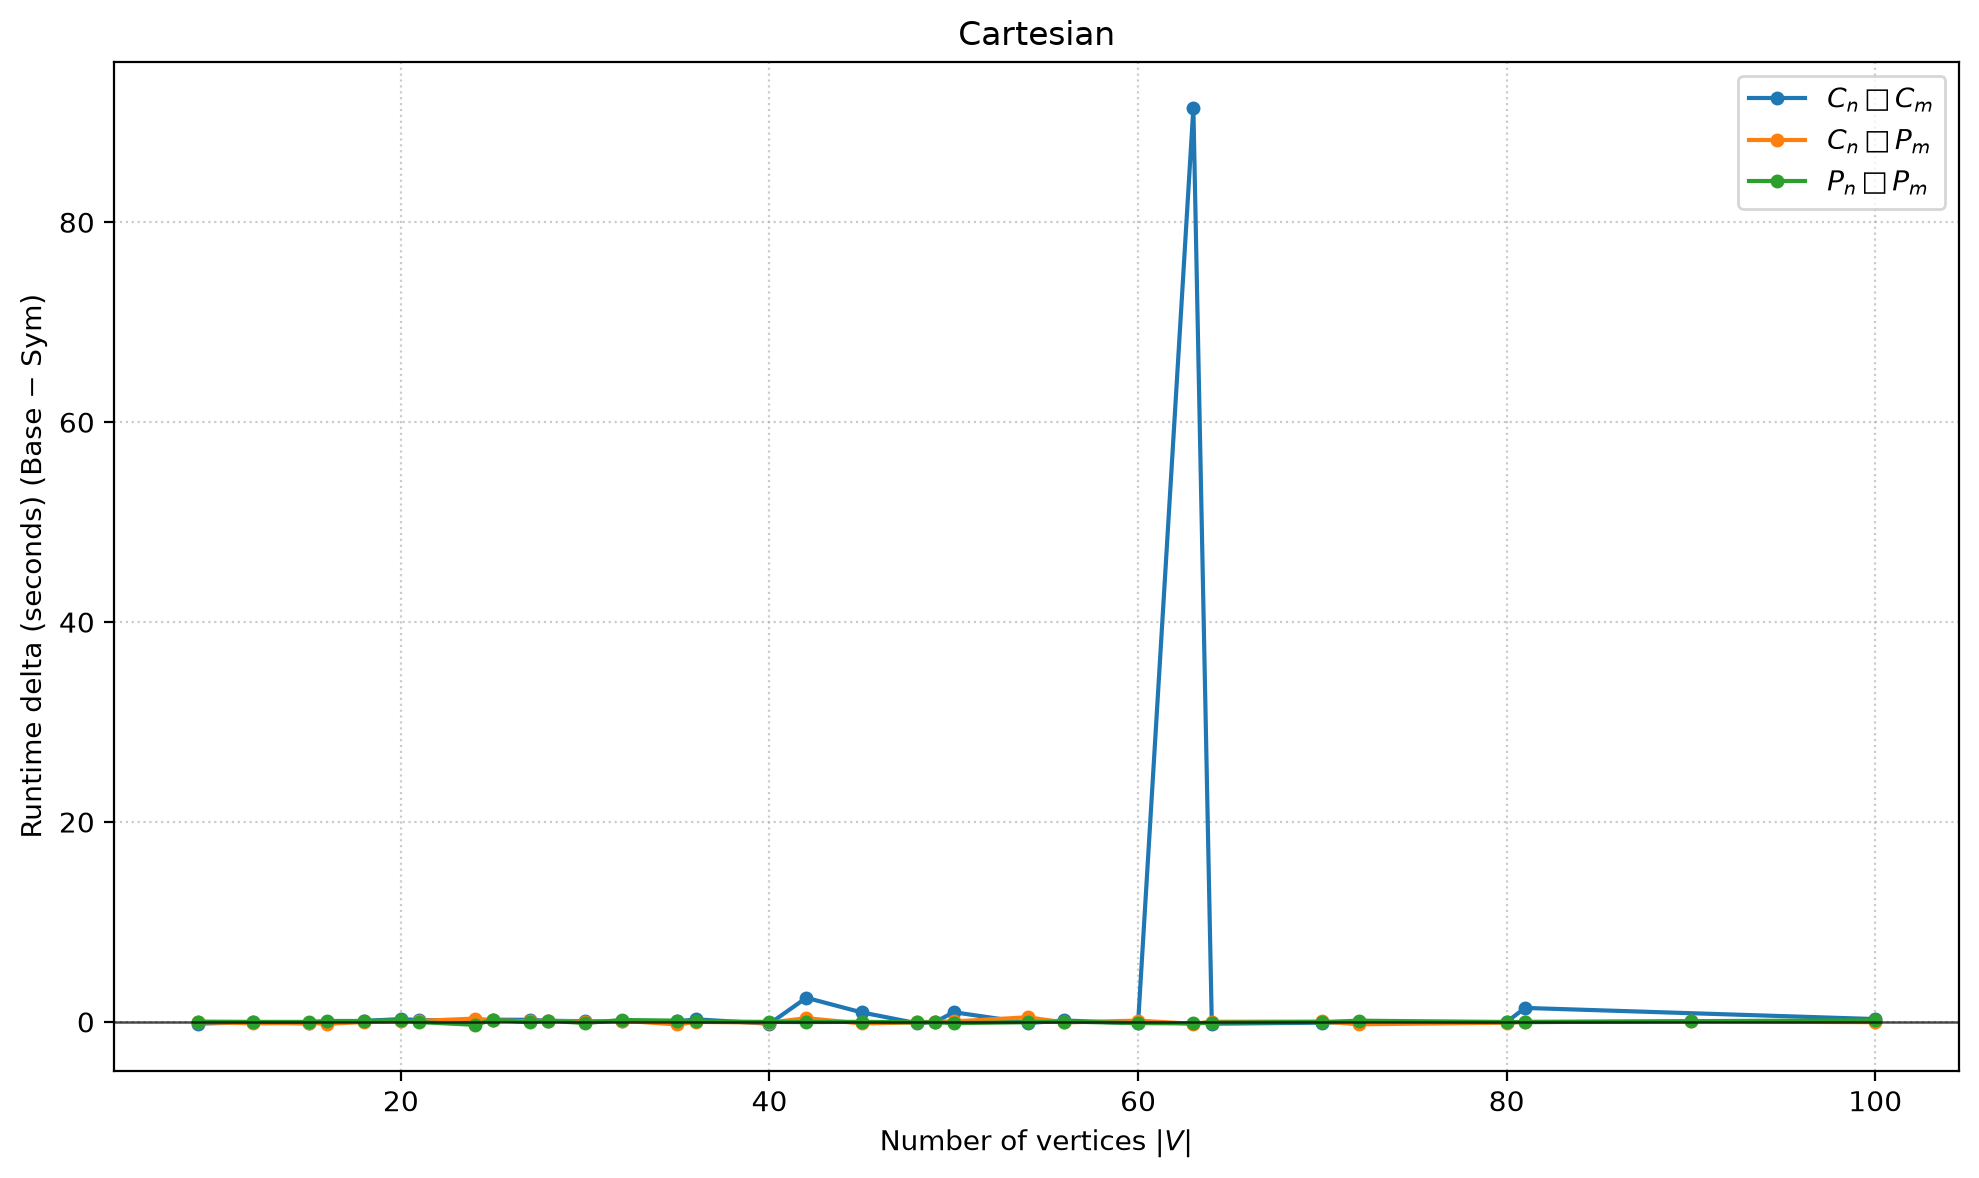
\includegraphics[width=0.49\linewidth]{paper/generated/products_main_r1_plots/delta_runtime_cartesian.png}
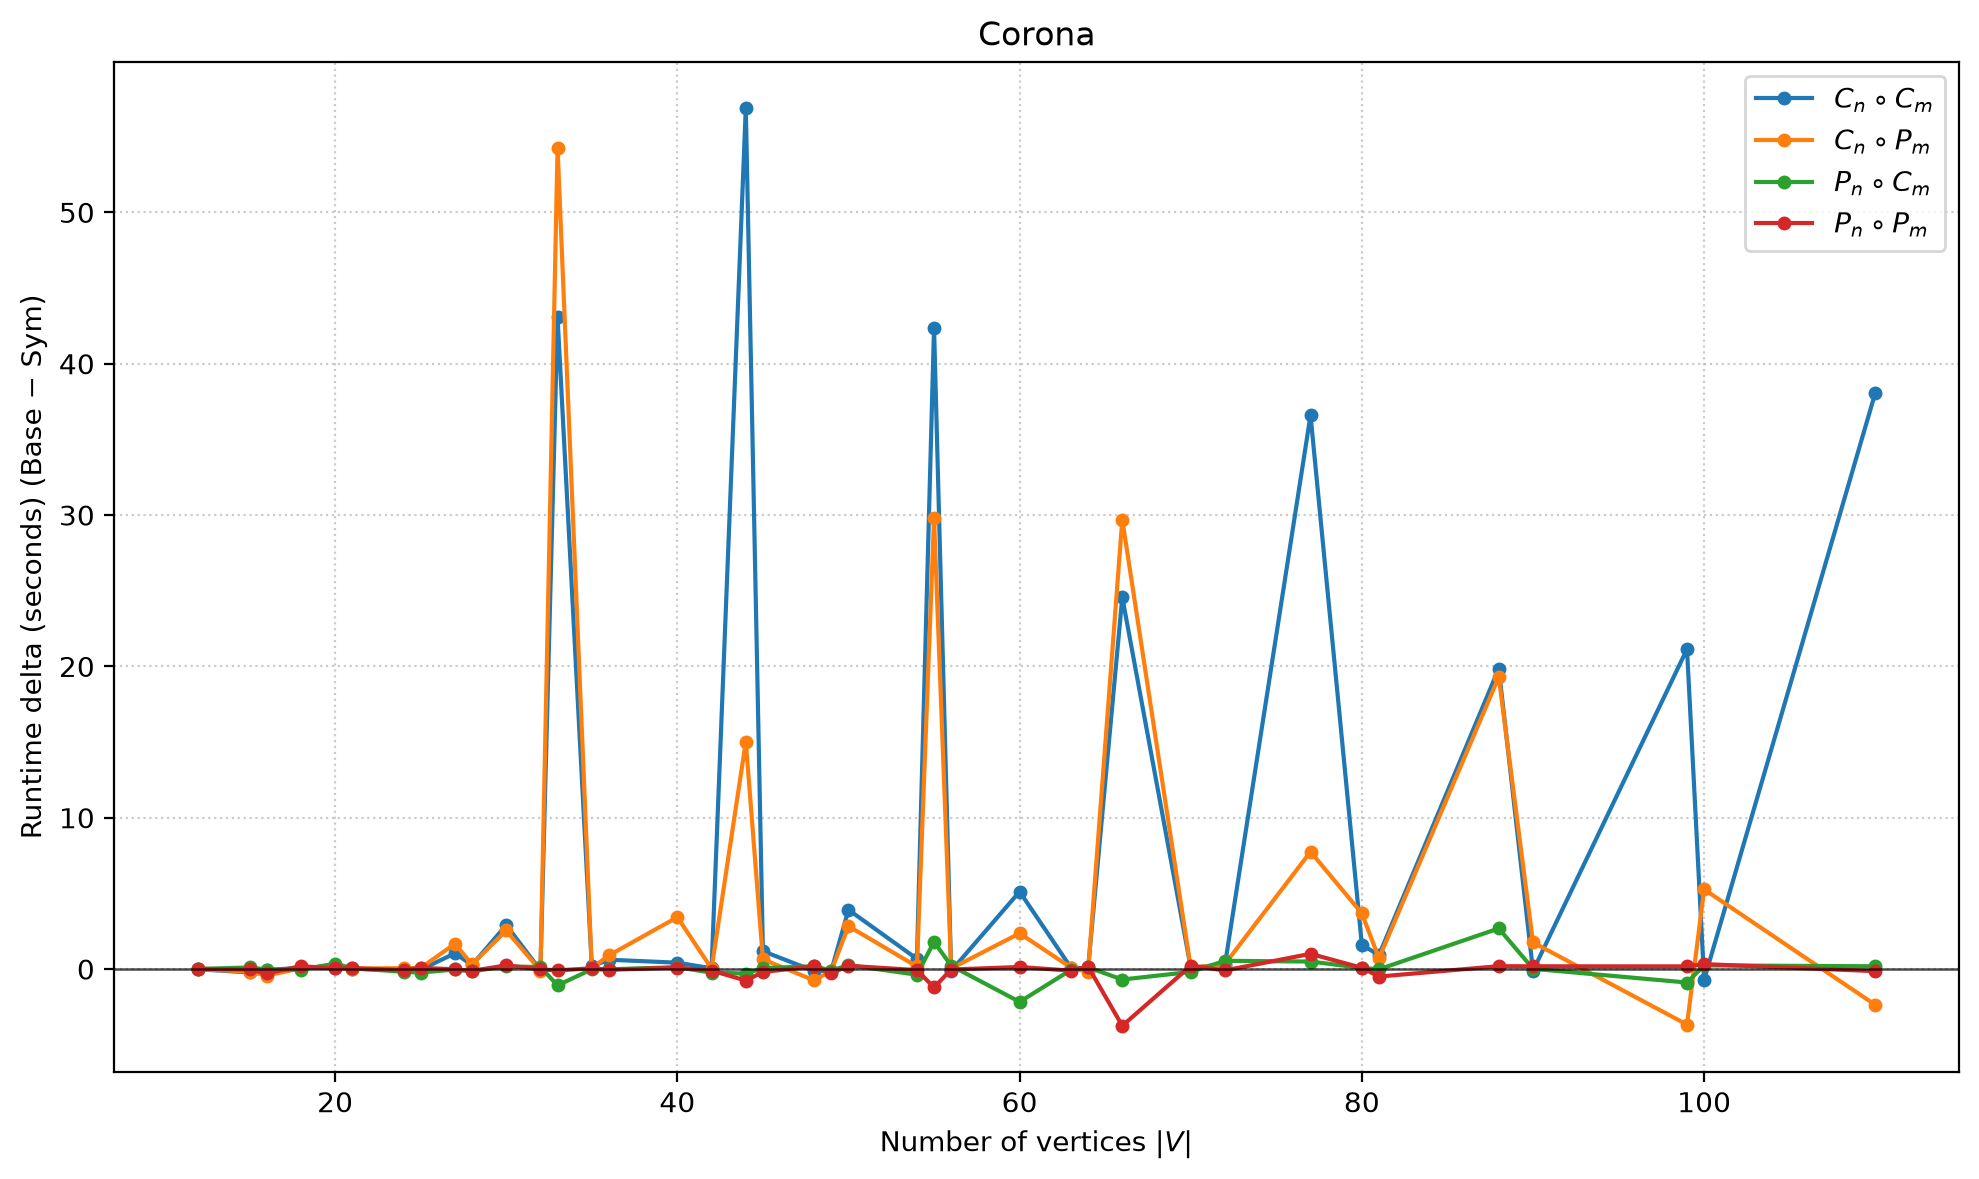
\includegraphics[width=0.49\linewidth]{paper/generated/products_main_r1_plots/delta_runtime_corona.png}
\caption{Runtime differences on graph products.}
\tablenote{Product runtimes: each curve represents a separate family; each
point is the mean difference over jointly OPT pairs in that family with the
same vertex count. Families are not pooled; the two unresolved pairs are excluded.}
\end{figure}
\begin{figure}[htbp]
\centering
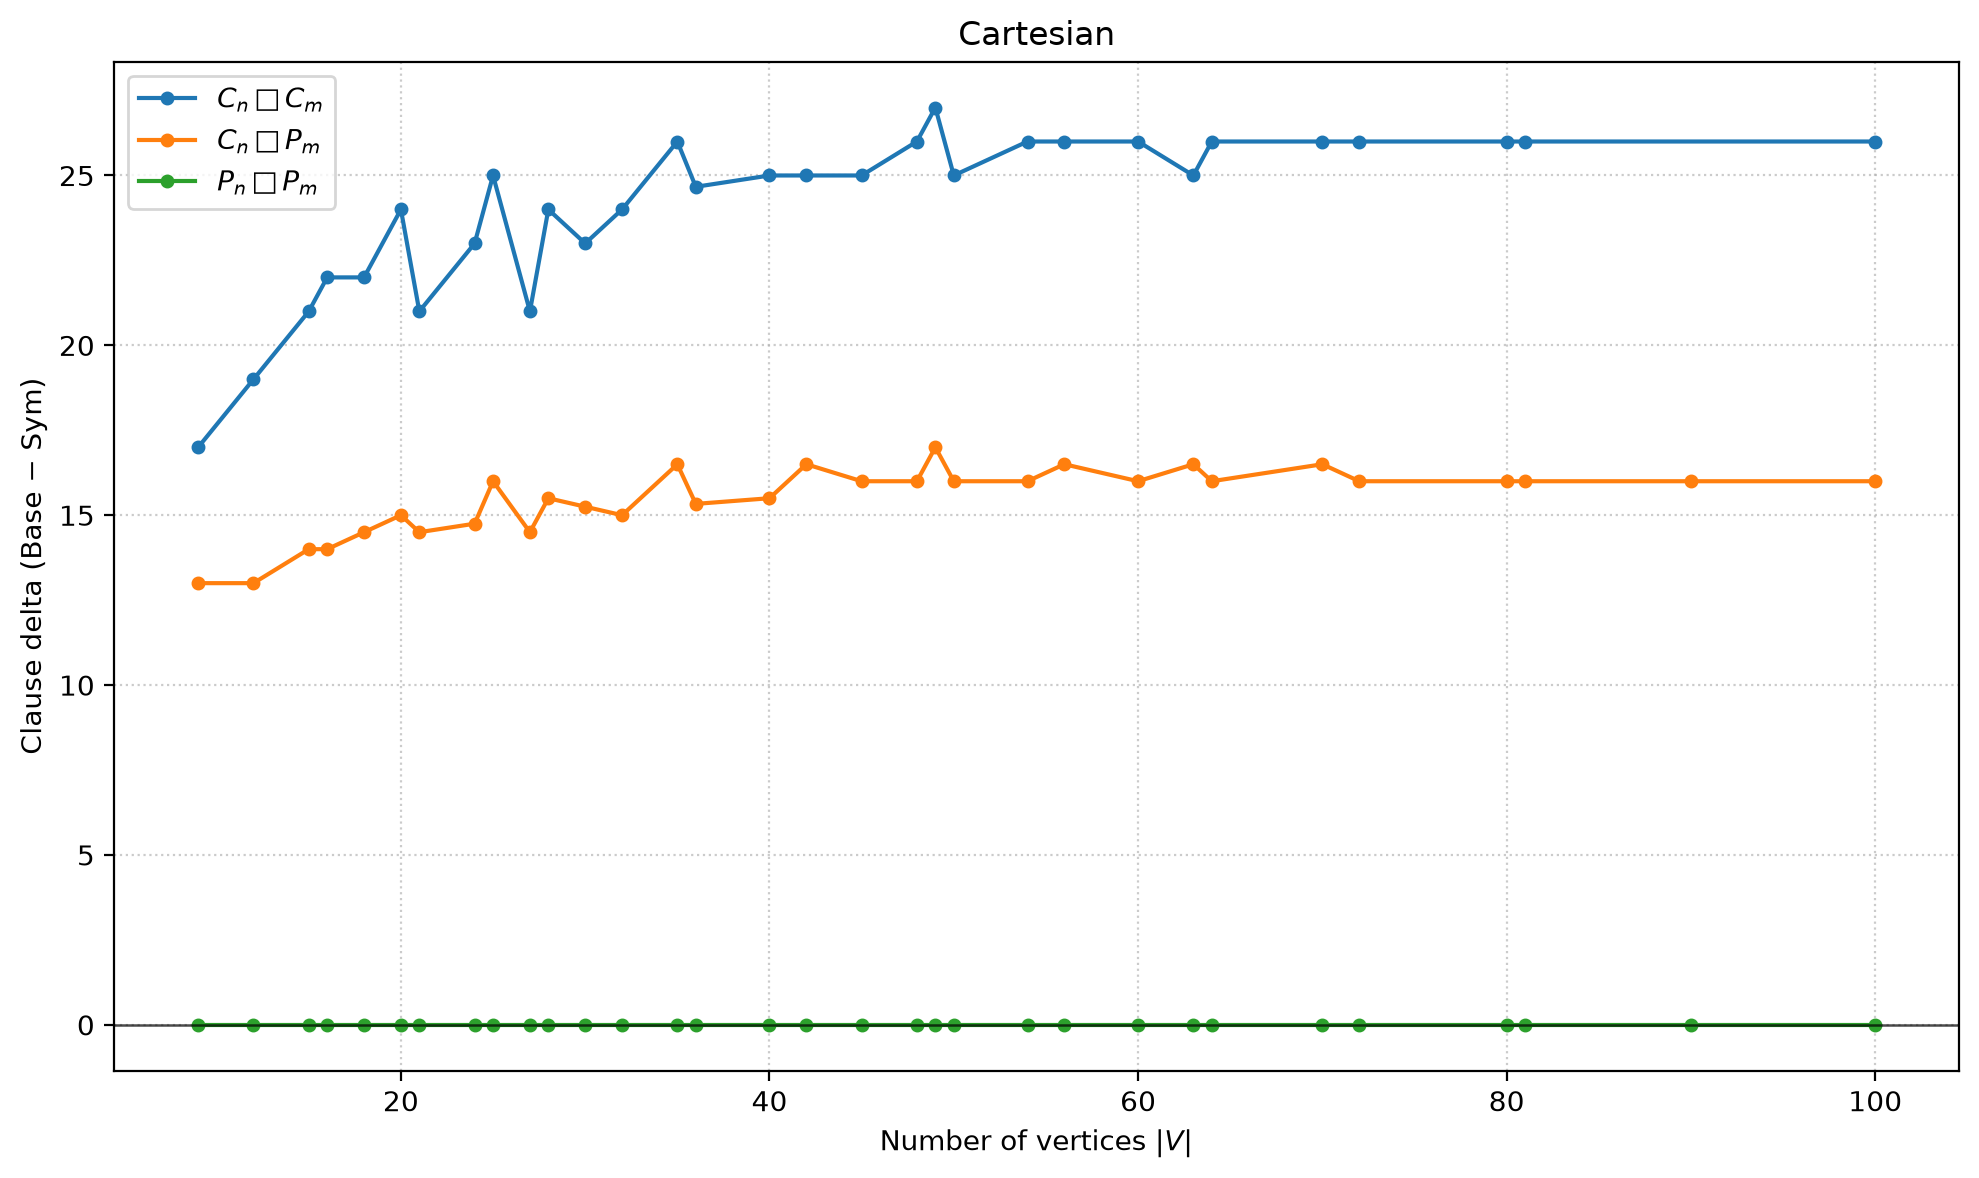
\includegraphics[width=0.49\linewidth]{paper/generated/products_main_r1_plots/delta_clauses_cartesian.png}
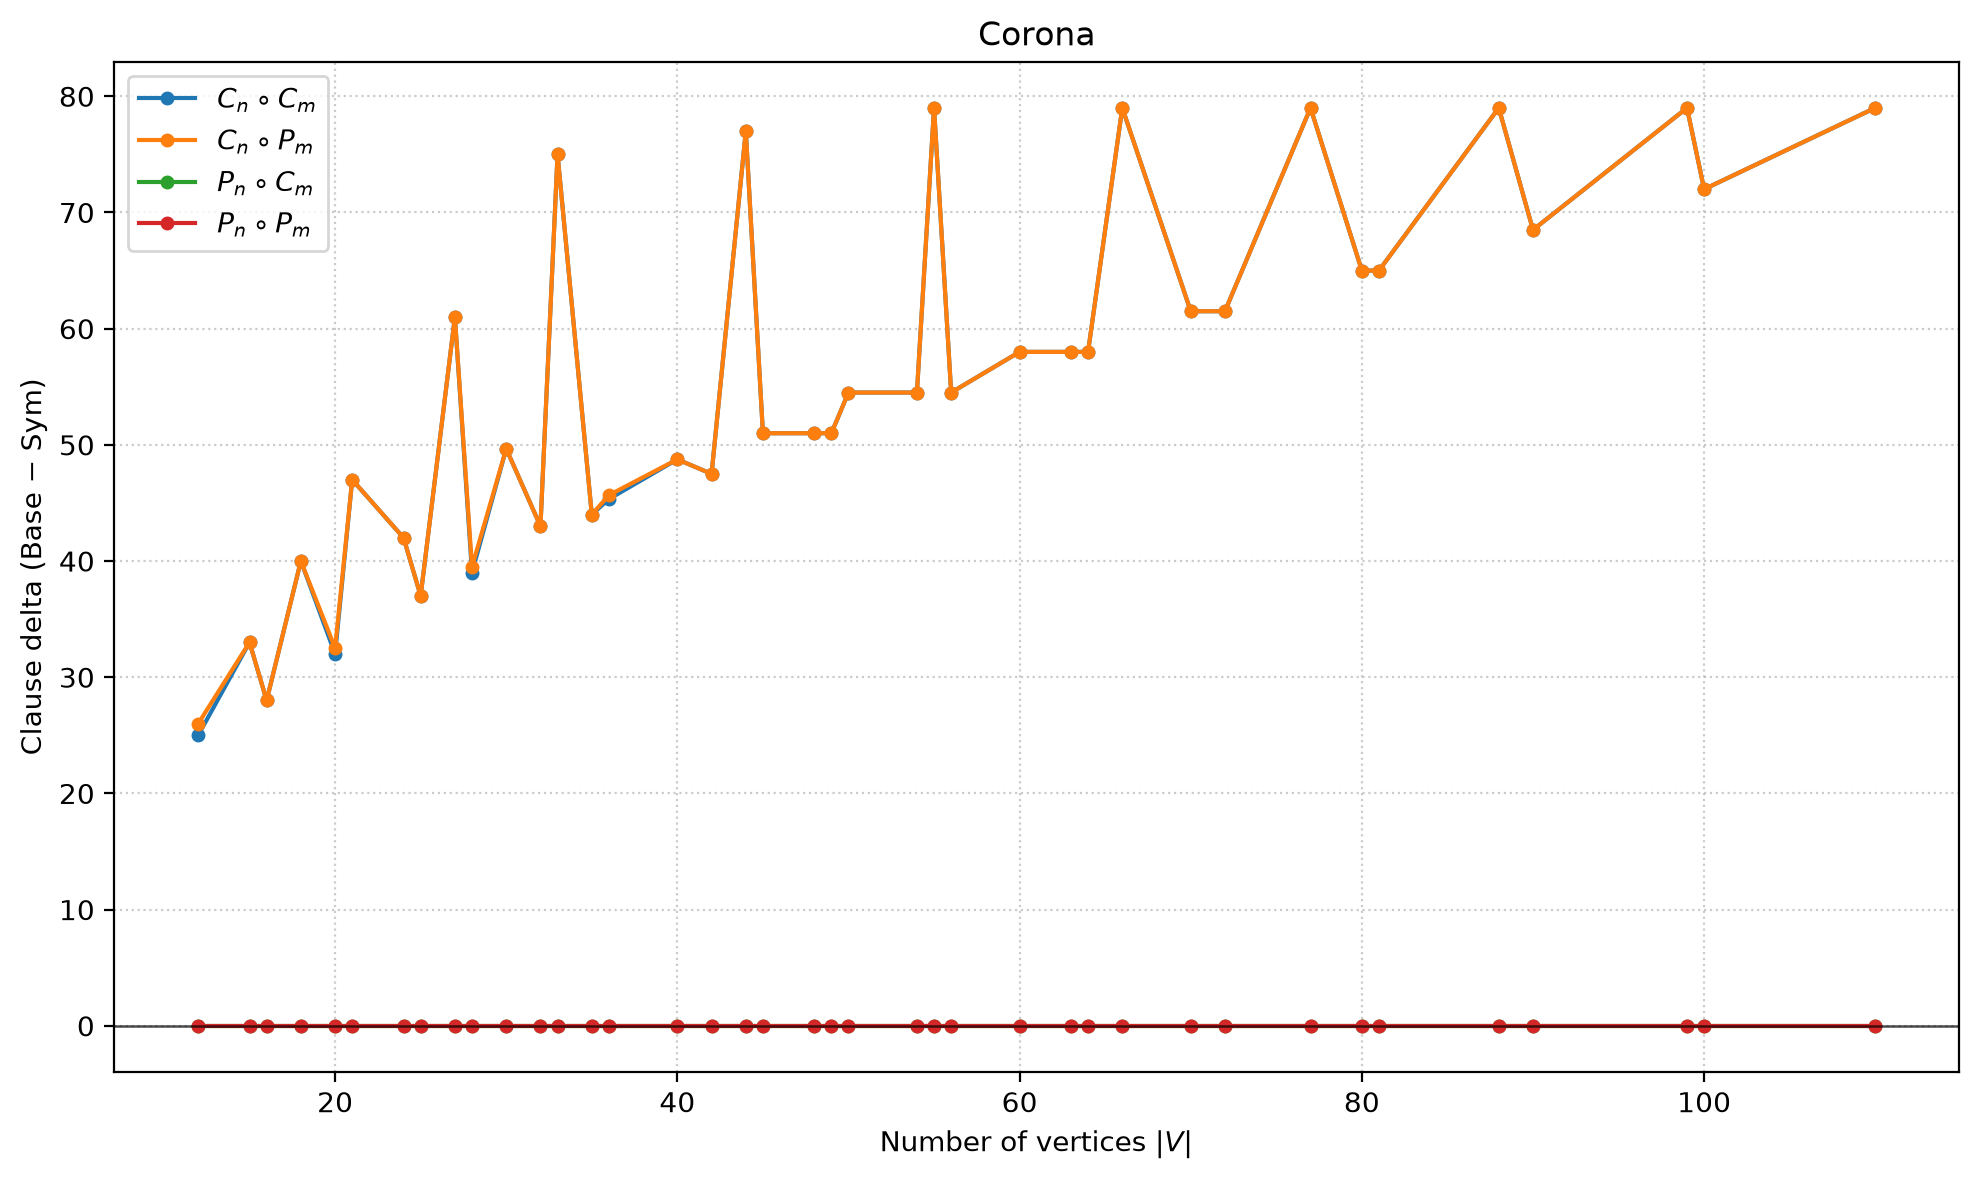
\includegraphics[width=0.49\linewidth]{paper/generated/products_main_r1_plots/delta_clauses_corona.png}
\caption{Clause differences on graph products.}
\tablenote{Product clauses: Base minus Sym at a common span after common
preprocessing, restricted to OPT/OPT pairs. Zero-valued curves may overlap
for families with no additional symmetry constraints.}
\end{figure}
\FloatBarrier

\subsection{Search counters and runtime components}
\begin{table}[H]
\caption{Glucose search counters.}
\centering\small\setlength{\tabcolsep}{4pt}% Generated from main runs; do not edit numbers manually.
\begin{tabular}{lrrrr}
\toprule
Family & Conflicts B & Conflicts S & Decisions B & Decisions S \\
\midrule
$C_n$ & 490 & 16 & 1014 & 304 \\
$C_n \mathbin{\square} C_m$ & 2822176 & 1561898 & 3703052 & 2086601 \\
$C_n \mathbin{\square} P_m$ & 62458 & 56542 & 96318 & 87201 \\
$P_n \mathbin{\square} P_m$ & 8282 & 8282 & 15175 & 15175 \\
$C_n \circ C_m$ & 28922138 & 19787058 & 35712056 & 24679416 \\
$C_n \circ P_m$ & 25550270 & 21037672 & 31640833 & 26452185 \\
$P_n \circ C_m$ & 15624199 & 15624199 & 19374024 & 19374024 \\
$P_n \circ P_m$ & 17120804 & 17120804 & 21294514 & 21294514 \\
\bottomrule
\end{tabular}

\tablenote{Total Glucose conflicts and decisions over completed span trials
on OPT/OPT pairs, including both SAT and UNSAT trials.}
\end{table}
\begin{table}[H]
\caption{Encoding and SAT-call times.}
\centering\small% Generated from main runs; do not edit numbers manually.
\begin{tabular}{lrrrr}
\toprule
Family & CNF build B & CNF build S & SAT B & SAT S \\
\midrule
$C_n$ & 0.0033 & 0.0027 & 0.0001 & 0.0000 \\
$C_n \mathbin{\square} C_m$ & 0.0718 & 0.0652 & 0.0241 & 0.0143 \\
$C_n \mathbin{\square} P_m$ & 0.0551 & 0.0558 & 0.0076 & 0.0069 \\
$P_n \mathbin{\square} P_m$ & 0.0454 & 0.0443 & 0.0012 & 0.0011 \\
$C_n \circ C_m$ & 0.0661 & 0.0629 & 0.3988 & 0.2334 \\
$C_n \circ P_m$ & 0.0629 & 0.0605 & 0.4020 & 0.2809 \\
$P_n \circ C_m$ & 0.0642 & 0.0740 & 0.0628 & 0.0683 \\
$P_n \circ P_m$ & 0.0647 & 0.0531 & 0.0808 & 0.1007 \\
\bottomrule
\end{tabular}

\tablenote{Median CNF-construction and internal SAT-call times in seconds,
summed within each search and then summarized over OPT/OPT pairs.}
\end{table}
Clause counts at a common span measure model size; total decisions/conflicts
measure work over all completed span trials. The two configurations may
visit different spans after finding different incumbents. Aggregate counters
therefore do not measure a single fixed-span call. Complete OPT-run counters
support search analysis but do not replace runtime measurements or repeated
runs. Counters from different backends are not automatically equivalent metrics.

\subsection{Reproduction and verification limits}
With the matching historical source version, \texttt{make report} checks
the two CSVs and their manifests/witnesses, reconstructs counts, generates
tables and figures, and compiles the manuscript. Raw results remain unchanged.
Benchmark resume requires matching configuration, source, schema, and environment;
a different budget or a retry of FEASIBLE rows requires a new run.

Tests use an exhaustive oracle on all atlas graphs through five vertices,
enumerate all assignments on three-vertex graphs, check multiple encoder-level
$h,k$ values, simplification equivalence, constructor reflections, and ILP
constraints. New Gurobi comparisons are reported in the main experimental
section; their times are not pooled with these SAT runs. After source changes,
the exporter refuses CNF reconstruction if hashes differ from the manifest.
The current PDF uses archived tables; old hashes are not changed to bypass checks.
Each main\_r1 instance has one measurement per configuration, so no variance
or confidence interval is estimated. Restricting timing to OPT/OPT pairs
can favor easier instances; these tables do not represent the complete domain
while timeout pairs remain.
